% !TeX spellcheck = de_DE
\documentclass{uebung_cs}
\usepackage{algo121}
\blattname{Wochenplan: Darstellung von Graphen, Breitensuche, Tiefensuche, Topologisches Sortieren}

%%%%%%%%%%%%%%%%%%%%%%%%%%%%%%%%%%%%%%%%%%%%%%%%%%%%%%%%%%%%%%%%%%%%%%%%%%%%


\begin{document}
\section*{Vorbereitung}
Lies CLRS Einleitung Teil VI, Kapitel 22.1 -- 22.4, sowie Appendix B.4 -- B.5 und schau das Video der Woche.

\section*{Dienstag}
\begin{aufgabe}[Darstellung, Eigenschaften und Algorithmen]\label{tue-first}
	Betrachte die Graphen in Abbildung \ref{ex1graph}.
	Löse die folgenden Teilaufgaben.
	\begin{enumerate}
		\item (\warmup) Gib die Adjazenzlisten und Adjazenzmatritzen für die Graphen 1 und 2 an.
		\item (\warmup) Tiefensuche wird auf Graph 1, beginnend von Knoten 0, ausgeführt.
		Die Adjazenzlisten sind hierbei aufsteigend sortiert.
		Gib den Tiefensuchebaum, Entdeckungsreihenfolge und -zeitpunkte an.
		\item (\warmup) Breitensuche wird auf Graph 1, beginnend von Knoten 0, ausgeführt.
		Die Adjazenzlisten sind hierbei aufsteigend sortiert.
		Gib den Breitensuchebaum und die Distanz zum Startknoten für alle Knoten an.
		\item Gib die Zusammenhangskomponenten der 3 Graphen an.
		\item Welche der 3 Graphen sind bipartit?
	\end{enumerate}
	%
	\begin{center}
		\begin{figure}[h]
			\begin{subfigure}[b]{0.33\textwidth}
				\hspace*{\fill}
				\scalebox{0.6}
				{
					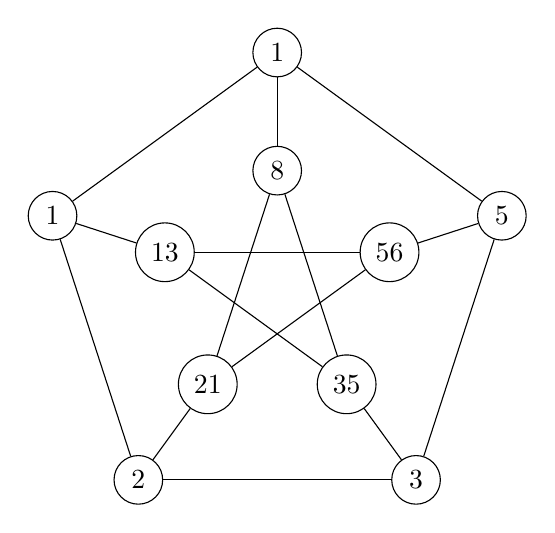
\begin{tikzpicture}
						% peterson graph labels
						\def\outer {1,1,2,3,5};
						\def\inner {8,13,21,35,56};
						% radii
						\def\outerRadius {3};
						\def\innerRadius {1.5};
						% petersen graph outer layer
						\foreach \label [count=\index] in \outer
						{
							\node[draw, circle] (outer_\index) at (\index*72+18:\outerRadius) {\label};
						}
						% petersen graph inner layer
						\foreach \label [count=\index] in \inner
						{
							\node[draw, circle] (inner_\index) at (\index*72+18:\innerRadius) {\label};
						}
						% petersen graph edges
						\foreach \current in {1,...,5}
						{
							% outer
							\pgfmathtruncatemacro{\next}{mod(\current,5)+1};
							\draw (outer_\current) -- (outer_\next);
							% inner
							\pgfmathtruncatemacro{\next}{mod(\current+1,5)+1};
							\draw (inner_\current) -- (inner_\next);
							% crossing
							\draw (outer_\current) -- (inner_\current);
						}
					\end{tikzpicture}
				}	
				\hspace*{\fill}
				\caption*{Graph 1}
			\end{subfigure}
			%
			\begin{subfigure}[b]{0.33\textwidth}
				\hspace*{\fill}
				\scalebox{0.6}
				{
					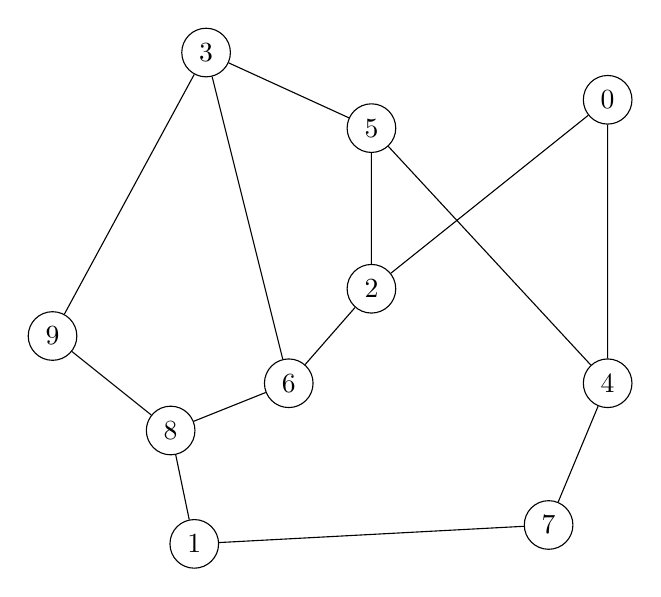
\begin{tikzpicture}
						% scale parameters
						\def\xscale {1.5};
						\def\yscale {1.2};
						% node labels
						\def\labels {9,8,1,6,3,5,2,0,4,7};
						% node xy coordinates
						\def\pos { (\xscale * 0   , 0     * \yscale)
								 , (\xscale * 1   , -1    * \yscale)
								 , (\xscale * 1.2 , -2.2  * \yscale)
								 , (\xscale * 2   , -0.5  * \yscale)
								 , (\xscale * 1.3 ,  3    * \yscale)
								 , (\xscale * 2.7 ,  2.2  * \yscale)
								 , (\xscale * 2.7 ,  0.5  * \yscale)
								 , (\xscale * 4.7 ,  2.5  * \yscale)
								 , (\xscale * 4.7 , -0.5  * \yscale)
								 , (\xscale * 4.2 , -2    * \yscale)
								 };
						% draw nodes and labels
						\foreach \coords [count=\index] in \pos
						{
							% node (v_\index) at \coords {\index};  % uncomment for debugging
							\node[draw, circle] (v_\index) at \coords {\phantom{0}};
						}
						\foreach \label [count=\index] in \labels
						{
							\node () at (v_\index) {\label};  % comment for debugging
						}
						% edges
						\draw  (v_2)  % path 1
							-- (v_3) 
							-- (v_10) 
							-- (v_9) 
							-- (v_8) 
							-- (v_7)
							-- (v_6)
							-- (v_9);
						\draw  (v_7)  % path 2
							-- (v_4)
							-- (v_2)
							-- (v_1)
							-- (v_5)
							-- (v_6);
						\draw  (v_5)
							-- (v_4);
					\end{tikzpicture}	
				}	
				\hspace*{\fill}
				\caption*{Graph 2}
			\end{subfigure}
			%
			\begin{subfigure}[b]{0.33\textwidth}
				\hspace*{\fill}
				\scalebox{0.6}
				{
					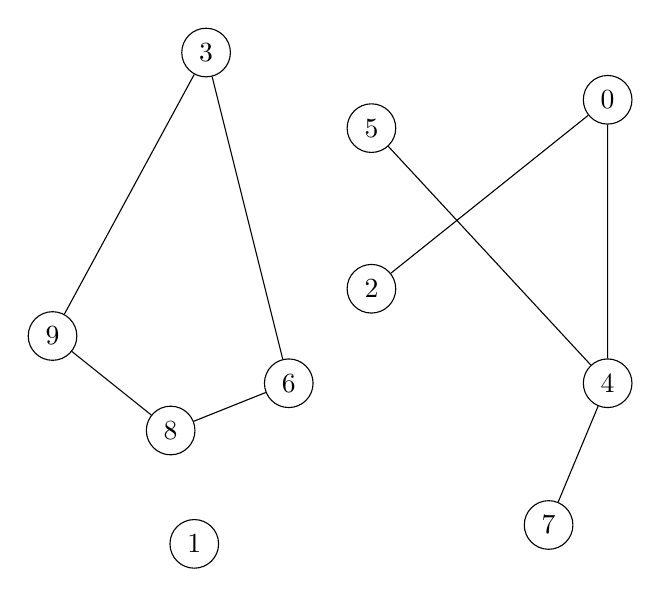
\begin{tikzpicture}
						% scale parameters
						\def\xscale {1.5};
						\def\yscale {1.2};
						% node labels
						\def\labels {9,8,1,6,3,5,2,0,4,7};
						% node xy coordinates
						\def\pos { (\xscale * 0   , 0     * \yscale)
								 , (\xscale * 1   , -1    * \yscale)
								 , (\xscale * 1.2 , -2.2  * \yscale)
								 , (\xscale * 2   , -0.5  * \yscale)
								 , (\xscale * 1.3 ,  3    * \yscale)
								 , (\xscale * 2.7 ,  2.2  * \yscale)
								 , (\xscale * 2.7 ,  0.5  * \yscale)
								 , (\xscale * 4.7 ,  2.5  * \yscale)
								 , (\xscale * 4.7 , -0.5  * \yscale)
								 , (\xscale * 4.2 , -2    * \yscale)
								 };
						% draw nodes and labels
						\foreach \coords [count=\index] in \pos
						{
							%\node (v_\index) at \coords {\index};  % uncomment for debugging
							\node[draw, circle] (v_\index) at \coords {\phantom{0}};
						}
						\foreach \label [count=\index] in \labels
						{
							\node () at (v_\index) {\label};  % comment for debugging
						}
						% edges
						\draw  (v_1)  % path 1
							-- (v_2) 
							-- (v_4) 
							-- (v_5)
							-- (v_1);
						\draw  (v_7)  % path 2
							-- (v_8)
							-- (v_9)
							-- (v_6);
						\draw  (v_10)
							-- (v_9);
					\end{tikzpicture}	
				}	
				\hspace*{\fill}
				\caption*{Graph 3}
			\end{subfigure}
			\caption{Graphen für Aufgabe 1. Graph 1 wird auch als \textit{Petersen-Graph} bezeichnet.}
			\label{ex1graph}
		\end{figure}
	\end{center}
\end{aufgabe}

\begin{aufgabe}[Buchstabenlabyrinth]
	Algolina und ihre kleine Schwester spielen das Buchstabenlabyrinth Spiel.
	In diesem Spiel wird, wie im Beispiel, eine $N\times N$ Matrix mit As und Bs gefüllt.
	Die Herausforderung ist es einen kürzesten Pfad von oben links nach unten rechts zu finden.
	Die Knoten auf dem Pfad müsssen dabei allerdings zwischen A und B alternieren, sprich die Buchstaben eines Pfades buchstabieren ABABABAB...
	Der Pfad darf immer nur horizontal und vertikal gehen, diagonale Bewegungen sind also nicht erlaubt.
	Im Beispiel sind die Buchstaben des kürzesten Pfads bold geschrieben.
	\begin{center}
		\begin{tabular}{ccccc}
			\textbf{A} & A & \textbf{A} & \textbf{B} & \textbf{A}\\
			\textbf{B} & B & \textbf{B} & B & \textbf{B}\\
			\textbf{A} & \textbf{B} & \textbf{A} & A & \textbf{A}\\
			A & B & B & B & \textbf{B}\\
			A & A & A & A & \textbf{A}
		\end{tabular}
	\end{center}
	Da die Schwestern sich nicht sicher sind, ob sie auch tatsächlich den kürzesten Weg gefunden haben wollen sie ein Programm schreiben, das es für sie beantwortet.
	Entwirf einen Algorithmus, der für eine, wie zuvor definierte, Matrix die Länge eines kürzsten Weges findet.
	Implementiere den Algorithmus in einer Programmiersprache deiner Wahl.
	%@Holger: Du wolltest ja eigentlich erstmal den Programmierteil aus den Übungen rausnehmen oder bring ich da was durcheinander?
\end{aufgabe}

\begin{aufgabe}[Tiefensuche mittels eines Stapels]
	Erkläre wie Tiefensuche rekursionslos mit einem Stapel implementiert werden kann.
\end{aufgabe}

\begin{aufgabe}[Wer nix weiß sucht einen Kreis]
	Entwirf einen Algorithmus, der feststellt ob ein Graph einen Kreis enthält.
	Wie schnell ist dein Algorithmus?
\end{aufgabe}

% #########################
% für aufgabe 6
% #########################
\begin{center}
	\begin{figure}[h]
		\begin{subfigure}[b]{0.24\textwidth}
			\hspace*{\fill}
			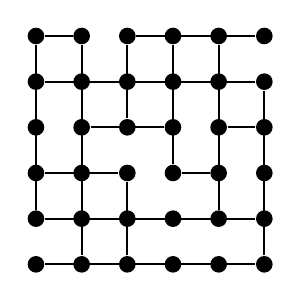
\begin{tikzpicture}
				\def\scale {0.58};
				% draw 6x6 node grid
				\foreach \x in {1,...,6}
				{
					\foreach \y in {1,...,6}
					{
						\node[fill=black, circle, inner sep=0pt, minimum size=6pt] (\x_\y) at (\scale * \x,\y * \scale) {};
					}
				}
				% horizontal edges
				\draw[thick] (1_1) -- (6_1);
				\draw[thick] (1_2) -- (6_2);
				\draw[thick] (1_3) -- (3_3);
				\draw[thick] (4_3) -- (5_3);
				\draw[thick] (2_4) -- (4_4);
				\draw[thick] (5_4) -- (6_4);
				\draw[thick] (1_5) -- (6_5);
				\draw[thick] (1_6) -- (2_6);
				\draw[thick] (3_6) -- (6_6);
				% vertical edges
				\draw[thick] (1_2) -- (1_6);
				\draw[thick] (2_1) -- (2_6);
				\draw[thick] (3_1) -- (3_3);
				\draw[thick] (3_4) -- (3_6);
				\draw[thick] (4_3) -- (4_6);
				\draw[thick] (5_2) -- (5_6);
				\draw[thick] (6_1) -- (6_5);
			\end{tikzpicture}	
			\hspace*{\fill}
			\caption{}
		\end{subfigure}
		\begin{subfigure}[b]{0.24\textwidth}
			\hspace*{\fill}
			\scalebox{0.5}
			{
				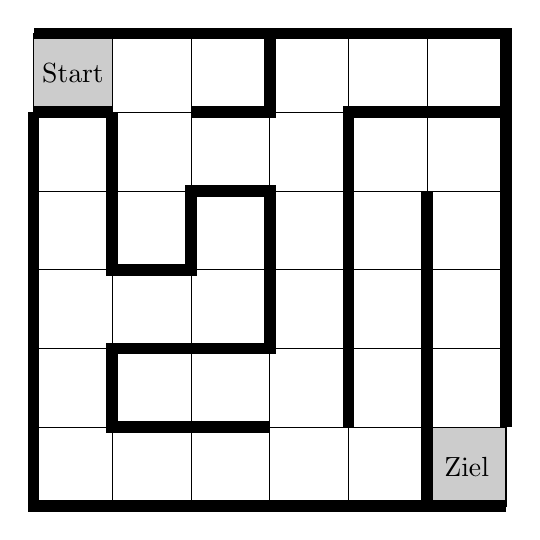
\begin{tikzpicture}
					% 6x6 grid
					\draw (0,0) grid (6,6);
					% target label backdrops
					\draw[fill=black!20] (5,1) rectangle (6,0);
					\draw[fill=black!20] (0,6) rectangle (1,5);
					% target labels
					\node () at (5.5,0.5) {Ziel};
					\node () at (0.5,5.5) {Start};                
	
					% ####################################
					%
					% toggle options
					% option (b): wall south to start
					\draw[line width=1.5mm] (0,5) -- (1,5);
					%
					% option (c): red filled rectangle and additional wall
					% \fill[red] (4,1) rectangle (5,0); \draw[line width=1.5mm] (4,0) -- (4,1);
					%
					% option (d) dashed red line
					% \draw[line width=1mm, dashed, red] (0.5,5.5) -- (0.5,0.5) -- (3.5,0.5) -- (3.5,4.5) -- (1.5,4.5) -- (1.5,5.5) -- (0.5,5.5);
					%
					% ####################################
	
					% walls
					\draw[line width=1.5mm]
								 (6,0)
							  -- (0,0)
							  -- (0,5);
					\draw[line width=1.5mm]
								 (1,5)
							  -- (1,3)
							  -- (2,3)
							  -- (2,4)
							  -- (3,4)
							  -- (3,2)
							  -- (1,2)
							  -- (1,1)
							  -- (3,1);
					\draw[line width=1.5mm]
								 (5,0)
							  -- (5,4);
					\draw[line width=1.5mm]
								 (4,1)
							  -- (4,5)
							  -- (6,5)
							  -- (6,1);
					\draw[line width=1.5mm]
								 (6,5)
							  -- (6,6)
							  -- (0,6);
					\draw[line width=1.5mm]
								 (3,6)
							  -- (3,5)
							  -- (2,5);
				\end{tikzpicture}    
			}	
			\hspace*{\fill}
			\caption{}
		\end{subfigure}
		\begin{subfigure}[b]{0.24\textwidth}
			\hspace*{\fill}
			\scalebox{0.5}
			{
				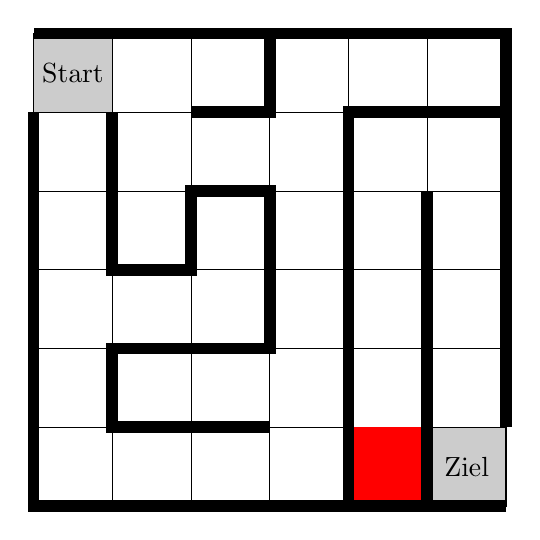
\begin{tikzpicture}
					% 6x6 grid
					\draw (0,0) grid (6,6);
					% target label backdrops
					\draw[fill=black!20] (5,1) rectangle (6,0);
					\draw[fill=black!20] (0,6) rectangle (1,5);
					% target labels
					\node () at (5.5,0.5) {Ziel};
					\node () at (0.5,5.5) {Start};                
	
					% ####################################
					%
					% toggle options
					% option (b): wall south to start
					%\draw[line width=1.5mm] (0,5) -- (1,5);
					%
					% option (c): red filled rectangle and additional wall
					\fill[red] (4,1) rectangle (5,0); \draw[line width=1.5mm] (4,0) -- (4,1);
					%
					% option (d) dashed red line
					% \draw[line width=1mm, dashed, red] (0.5,5.5) -- (0.5,0.5) -- (3.5,0.5) -- (3.5,4.5) -- (1.5,4.5) -- (1.5,5.5) -- (0.5,5.5);
					%
					% ####################################
	
					% walls
					\draw[line width=1.5mm]
								 (6,0)
							  -- (0,0)
							  -- (0,5);
					\draw[line width=1.5mm]
								 (1,5)
							  -- (1,3)
							  -- (2,3)
							  -- (2,4)
							  -- (3,4)
							  -- (3,2)
							  -- (1,2)
							  -- (1,1)
							  -- (3,1);
					\draw[line width=1.5mm]
								 (5,0)
							  -- (5,4);
					\draw[line width=1.5mm]
								 (4,1)
							  -- (4,5)
							  -- (6,5)
							  -- (6,1);
					\draw[line width=1.5mm]
								 (6,5)
							  -- (6,6)
							  -- (0,6);
					\draw[line width=1.5mm]
								 (3,6)
							  -- (3,5)
							  -- (2,5);
				\end{tikzpicture}    
			}	
			\hspace*{\fill}
			\caption{}
		\end{subfigure}
		\begin{subfigure}[b]{0.24\textwidth}
			\hspace*{\fill}
			\scalebox{0.5}
			{
				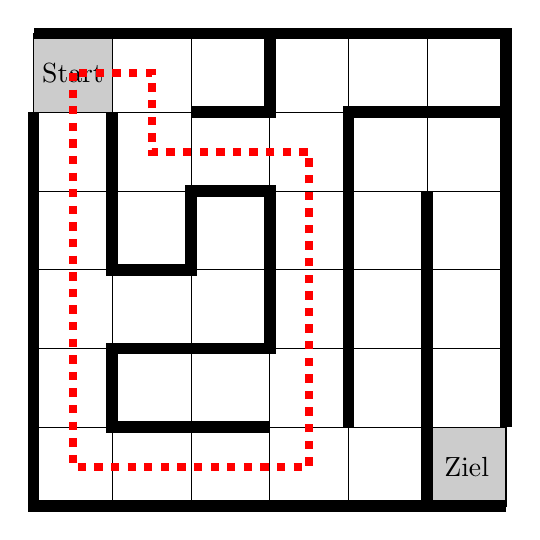
\begin{tikzpicture}
					% 6x6 grid
					\draw (0,0) grid (6,6);
					% target label backdrops
					\draw[fill=black!20] (5,1) rectangle (6,0);
					\draw[fill=black!20] (0,6) rectangle (1,5);
					% target labels
					\node () at (5.5,0.5) {Ziel};
					\node () at (0.5,5.5) {Start};                
	
					% ####################################
					%
					% toggle options
					% option (b): wall south to start
					%\draw[line width=1.5mm] (0,5) -- (1,5);
					%
					% option (c): red filled rectangle and additional wall
					% \fill[red] (4,1) rectangle (5,0); \draw[line width=1.5mm] (4,0) -- (4,1);
					%
					% option (d) dashed red line
					\draw[line width=1mm, dashed, red] (0.5,5.5) -- (0.5,0.5) -- (3.5,0.5) -- (3.5,4.5) -- (1.5,4.5) -- (1.5,5.5) -- (0.5,5.5);
					%
					% ####################################
	
					% walls
					\draw[line width=1.5mm]
								 (6,0)
							  -- (0,0)
							  -- (0,5);
					\draw[line width=1.5mm]
								 (1,5)
							  -- (1,3)
							  -- (2,3)
							  -- (2,4)
							  -- (3,4)
							  -- (3,2)
							  -- (1,2)
							  -- (1,1)
							  -- (3,1);
					\draw[line width=1.5mm]
								 (5,0)
							  -- (5,4);
					\draw[line width=1.5mm]
								 (4,1)
							  -- (4,5)
							  -- (6,5)
							  -- (6,1);
					\draw[line width=1.5mm]
								 (6,5)
							  -- (6,6)
							  -- (0,6);
					\draw[line width=1.5mm]
								 (3,6)
							  -- (3,5)
							  -- (2,5);
				\end{tikzpicture}    
			}	
			\hspace*{\fill}
			\caption{}
		\end{subfigure}
		\caption{}
		\label{ex6mazes}
	\end{figure}
\end{center}

% #########################
% für aufgabe 7
% #########################
\begin{center}
	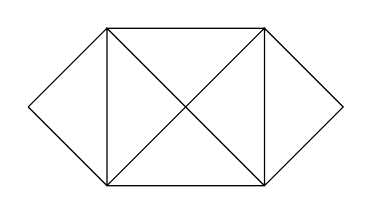
\begin{tikzpicture}
		% graph 1 has an euler tour :D
		\draw (0,0) -- (1,-1) -- (2,0) -- (3,-1) -- (4,0) -- (3,1) -- (3,-1) -- (1,-1) -- (1,1) -- (2,0) -- (3,1) -- (1,1) -- (0,0);
	\end{tikzpicture}
	%
	\hspace{1.5cm}
	%
	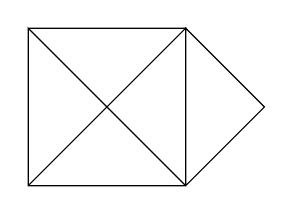
\begin{tikzpicture}
		% graph 2 has an euler tour :D
		\draw (1,-1) -- (2,0) -- (3,-1) -- (4,0) -- (3,1) -- (3,-1) -- (1,-1) -- (1,1) -- (2,0) -- (3,1) -- (1,1);
	\end{tikzpicture}
	%
	\hspace{1.5cm}
	%
	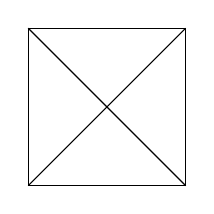
\begin{tikzpicture}
		% graph 3 does not :D
		\draw (1,-1) -- (3,-1) -- (3,1) -- (1,1) -- (1,-1);
		\draw (1,-1) -- (3,1);
		\draw (1,1) -- (3,-1);
	\end{tikzpicture}
\end{center}

\end{document}
